\section*{Aufgabe 3}
\subsection*{a)}

Die mittels kleinste Quadrate ermittelten Parameter sind:\\
3.63230696e-05	\\
-9.86645792e-04	\\
1.02008069e-02	\\
-4.74531133e-02	\\
8.25540287e-02	\\
2.90985385e-05	\\
1.09489710e-01	\\


\begin{figure}[H]
  \centering
  \includegraphics[width=\textwidth]{./Python/Regulierungsstärke0.0.pdf}
  \caption{kleinste Quadrate Regulierung $\alpha = 0$}
\end{figure}

\subsection*{b)}
\begin{figure}[H]
  \centering
  \includegraphics[width=\textwidth]{./Python/Regulierungsstärke0.1.pdf}
  \caption{kleinste Quadrate Regulierung $\alpha = 0.1$}
\end{figure}

\begin{figure}
  \centering
  \includegraphics[width=\textwidth]{./Python/Regulierungsstärke0.3.pdf}
  \caption{kleinste Quadrate Regulierung $\alpha = 0.3$}
\end{figure}

\begin{figure}
  \centering
  \includegraphics[width=\textwidth]{./Python/Regulierungsstärke0.7.pdf}
  \caption{kleinste Quadrate Regulierung $\alpha = 0.7$}
\end{figure}

\begin{figure}
  \centering
  \includegraphics[width=\textwidth]{./Python/Regulierungsstärke3.pdf}
  \caption{kleinste Quadrate Regulierung $\alpha = 3$}
\end{figure}

\begin{figure}
  \centering
  \includegraphics[width=\textwidth]{./Python/Regulierungsstärke10.pdf}
  \caption{kleinste Quadrate Regulierung $\alpha = 10$}
\end{figure}

\subsection*{c)}

\begin{figure}
  \centering
  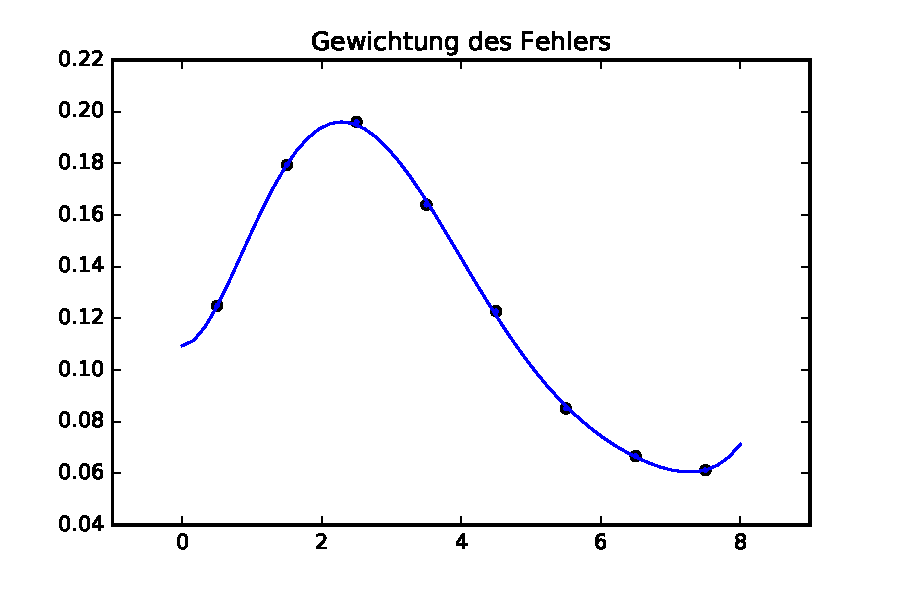
\includegraphics[width=\textwidth]{./Python/gewichtung.pdf}
  \caption{Der mittels Fehler des Mittelwerts berechneter Fit}
\end{figure}
